\section{Introdução}
\label{sec:introducao_formulacao_problema}

A proposta desta pesquisa de Mestrado consiste na abordagem do problema da dinâmica e controle de órbita e atitude de uma \gls{emtr} injetada em uma missão de Rendezvous and Docking or Berthing (RVD/B -- Encontro, Acoplamento ou Ancoragem).
A solução desse problema envolve a modelagem matemática da dinâmica orbital e da atitude da espaçonave, considerando as representações do movimento em duas configuração, absoluta (no referencial ECI) e relativa (referencial \gls{lvlh}).
O movimento relativo refere-se ao movimento entre as espaçonaves, além disso, o sistema de coordenadas orbital LVLH é definido na origem do centro de massa do alvo e segue com a órbita.

A formulação do problema de controle aplica-se a ambas representações do movimento no ECI e LVLH, para órbita e atitude, nas versões não-linear e linerarizada das equações do movimento relativo.
Um aspecto característico das missões de RVD/B é que o controle orbital feito pelo lançador, injeta o perseguidor em uma órbita próxima à da espaçonave alvo. 
Nessas condições, eventuais desvios do plano orbital da espaçonave perseguidora em relação ao da espaçonave alvo exigem correções, de modo a preservar a coplanaridade entre as órbitas dentro de limites que não comprometam a missão de RVD/B. 
A órbita final que antecede a aproximação de longa distância, deve ser estável e adequada para se ter início às manobras de fase (de longa e de curta distância), conforme a nomenclatura de \cite{fehse2003}, é ilustrada na Figura \eqref{fig:orbita_fase}.
% órbita de fase (\emph{phasing orbit})

% estável (na matematica). Derivada muda de 0 para inflexão, são pontos críticos, podendo ser estáveis ou não. Se for estável, ele volta; se não for, ele não volta.
% órbita estável = não será tão sensível em relação as perturbações; mantém a órbita de forma consistente por um determinado período de tempo, caso for longa demais, pode sofrer em demasiado com as perturbações.
% adequada = proxima para a manobra de phasing (que procura angulo adequado). está proximo o suficiente para as manobras relacionadas ao RVDB.

\begin{figure}[ht]
\centering
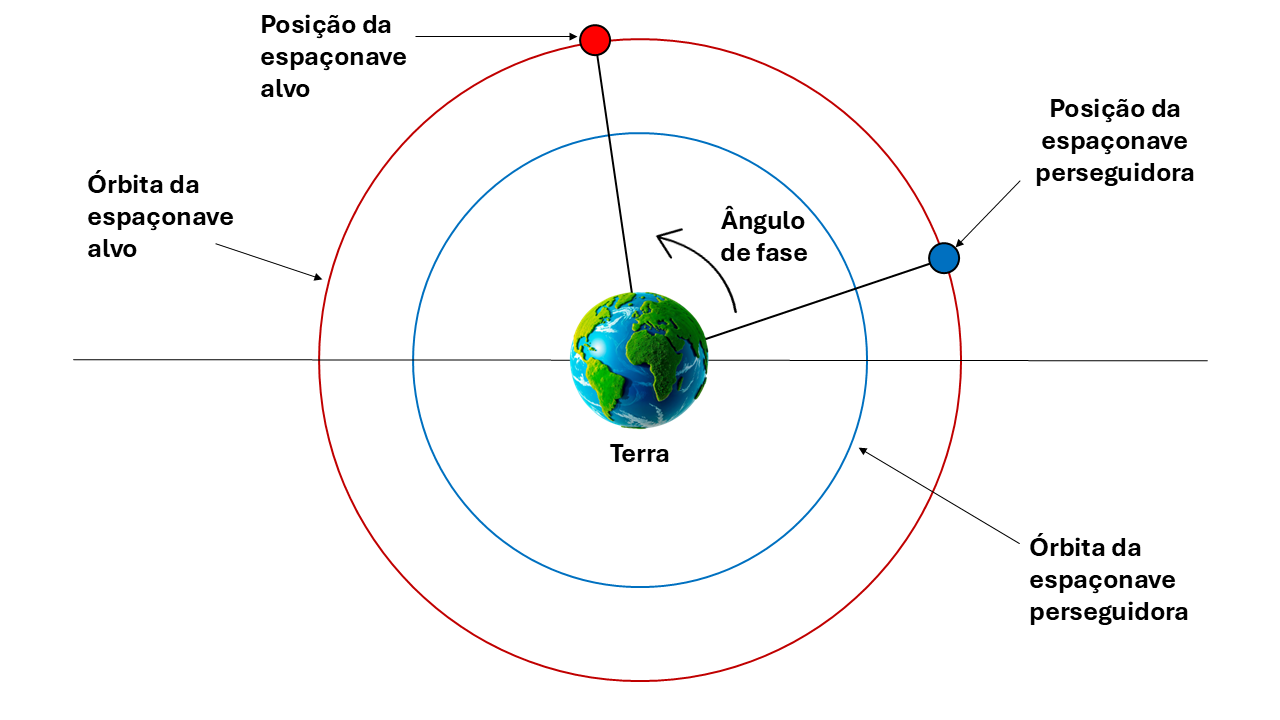
\includegraphics[width=1\linewidth]{3 Formulacao matematica/Imagens/Orbita de fase.png}
\caption{Órbita de fase, figura adaptada de \cite{fehse2003}.}
\label{fig:orbita_fase}
\end{figure}

Terminando as manobras de longa distância, inicia-se a abordagem do movimento relativo, para as das monobras de curta distância
A espaçonave alvo é assumida como não colaborativa, no sentido de não contribuir para o controle ou para o êxito das operações de RVD/B, portanto, para que ocorra o sucesso da missão, é necessário que a atitude relativa seja nula, isto é, que a atitude da espaçonave perseguidor coincida com a da espaçonave alvo.
Nesta pesquisa assume-se que o movimento relativo seja considerado a partir da aproximação de longa distância.
Em consonância com o problema de RVD/B, a análise dinâmica usa a modelagem matemática representada no referencial absoluto (ECI), ao passo que o movimento relativo é utilizado na fase de aproximação de curta distância e de aproximação de proximidade.
% Inicialmente, a análise dinâmica do movimento é conduzida no referencial absoluto, abrangendo as fases desde o lançamento até a execução da transferência orbital. Nesse estágio, a dinâmica orbital do alvo é descrita em relação ao sistema inercial geocêntrico, até que a espaçonave complete a manobra de transferência e se estabeleça em uma órbita próxima à do alvo.
% A partir dessa fase, quando as condições de fase e distância relativa são atendidas, passa-se a empregar a formulação do movimento relativo entre as naves.
% Nas fases de aproximação de curta duração e de proximidade, quando são realizadas as correções de órbita e de atitude até a conclusão da operação de acoplamento ou ancoragem, utiliza-se o modelo matemático da dinâmica relativa.
% Nesse contexto, o movimento relativo é descrito no referencial orbital LVLH (\emph{Local-Vertical-Local-Horizontal}).

A seguir será apresentada a formulação matemática necessária para descrever a dinâmica orbital associada às missões de RVD/B.
Serão descritas as equações fundamentais do movimento orbital e as manobras que estruturam a sequência de aproximação entre as espaçonaves.